\section{Clase 3 - Pr\'actica 2 (Ecuaciones diferenciales - Problema de valores iniciales)}

$$ 
	\begin{cases}
        y'(x) = f(x, y(x)), \ a \leq x \leq b\\
        y(a) = y_{0}\\
    \end{cases}
$$

\textit{Ejemplo}:

$$ 
	\begin{cases}
        y'(x) = y\\
        y(0) = 1\\
    \end{cases}
$$

$$\frac{dy}{dx} = x \Rightarrow dy = ydx \Rightarrow \int \frac{dy}{y} = \int dx \Rightarrow \ln(y) = x + \text{cte} \Rightarrow y = e^{x + \text{cte}} = e^{x}e^{\text{cte}} = ke^{x},\ k > 0$$

Como $y(0) = 1 = ke^{0} \Rightarrow k = 1$, luego:

$$y(x) = e^{x}$$

\underline{Teorema}: Si $f$ es continua en $I \times \mathbb{R},\ I = [a, b]$ y $f$ es Lipschitz en la segunda variable $(\exists \ \text{cte}\ L\ / \ |f(x, u) - f(x, v)| \leq L|u - v|)$ cualquiera sea $y_{0} \in \mathbb{R}$, existe una \'unica soluci\'on diferenciable $y(x)$ del problema.\\

\underline{Corolario}: Si $\bigg|\frac{\partial f}{\partial y}(x, y)\bigg| \leq k,\ x \in I,\ y \in \mathbb{R}$, entonces existe una \'unica soluci\'on

$$|f(x, u) - f(x, v)| = \bigg|\frac{\partial f}{\partial y}(x, \theta)(u - v)\bigg| \leq k|u - v|$$

con $\theta$ en un intervalo de extremos $u$ y $v$.\\

\subsection{M\'etodo de Euler}

Dados $y(a)$ y $f$, tomando $x_{0} = a, \cdots, x_{N} = b$ puntos equiespaciados, la recta tangente en $(x_{0}, y(x_{0}))$ es:

$$y(x) = y(x_{0}) + y'(x_{0})(x - x_{0})$$

Evaluamos en $x_{1}$:

$$y_{1} = y(x_{1}) = y(x_{0}) + y'(x_{0})(x_{1} - x_{0}) = y(x_{0}) + f(x_{0}, y(x_{0}))(x_{1} - x_{0}) = y(x_{0}) + f(x_{0}, y(x_{0}))h$$

Con este dato, evaluamos ahora en $x_{2}$:

$$y_{2} = y(x_{2}) = y(x_{1}) + y'(x_{1})(x_{2} - x_{1}) = y_{1} + f(x_{1}, y(x_{1}))h$$

En general:

$$ 
	\begin{cases}
        y_{i + 1} = y_{i} + hf(x_{i}, y_{i}),\ i = 0, \cdots, N - 1\\
        y_{0} = y(a) = y(x_{0})\\
    \end{cases}
$$

El resultado de los m\'etodos es una tira de puntos, despu\'es aproximamos $y(x)$ interpolando.\\

Vamos a proponer y analizar f\'ormulas de aproximaci\'on de un paso:

$$y_{i + 1} = y_{i} + h\phi(x_{i}, y_{i}, h)$$

en particular, en Euler, $\phi = f(x_{i}, y_{i})$.\\

\textit{Python}: Euler

$$ 
	\begin{cases}
        y'(t) = -y(t),\ t \in [0, 2]\\
        y(0) = 1\\
    \end{cases}
$$

\begin{verbatim}
	import numpy as np
	import matplotlib.pyplot as plt
	
	def f(t, y):
	    return (-y)
		
	def Euler(a, b, N, f, y0):
	    h = (b - a) / N
	    t = np.linspace(a, b, N + 1)
	    y = np.zeros(N + 1)
	    y[0] = y0
		
	    for k in range(1, N + 1):
	        y[k] = y[k - 1] + f(t[k - 1], y[k - 1]) * h
		
	    return (t, y)
		
	a = 0
	b = 2
	N = 10
	y0 = 1
	
	t, y = Euler(a, b, N, f, y0)
	
	plt.plot(t, y, 'o', label = 'Euler', markersize = 3)
	
	t_exacta = np.linspace(a, b, 100)
	y_exacta = np.exp(t_exacta)
	
	plt.plot(t_exacta, y_exacta, label = 'exacta')
	plt.grid()
	plt.legend()
	plt.show()
\end{verbatim}

\begin{figure}[H]
  \centering
  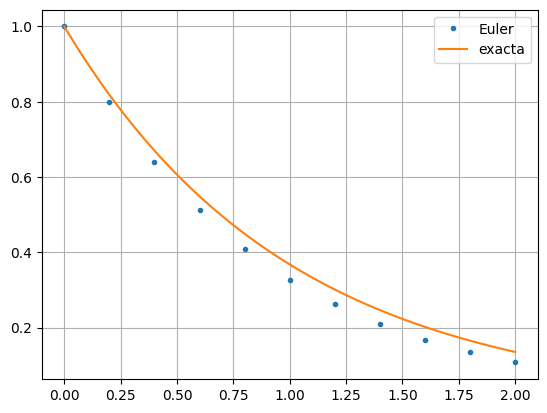
\includegraphics[width=0.6\linewidth]{Clase3_Practica2/euler_c3p2.png}
\end{figure}

\subsection{M\'etodo de Taylor de orden $k$}

$$y(x) \approx y(x_{0}) + y'(x_{0})(x - x_{0}) + y''(x_{0})\frac{(x - x_{0})^{2}}{2!} + \cdots + y^{k}(x_{0})\frac{(x - x_{0})^{k}}{k!} + \mathcal{O}((x - x_{0})^{k + 1})$$

Si $k = 1$, el m\'etodo de Taylor de orden 1 es Euler:

$$y(x) \approx y(x_{0}) + y'(x_{0})(x - x_{0}) = y(x_{0}) + f(x_{0}, y(x_{0}))$$

Si $k = 2$:

$$y(x) \approx y(x_{0}) + y'(x_{0})(x - x_{0}) + y''(x_{0})\frac{(x - x_{0})^{2}}{2!}$$

$$y'(x) = f(x, y(x)) \Rightarrow y''(x) = \frac{\partial f}{\partial x}(x, y(x))1 + \frac{\partial f}{\partial y}(x, y(x))y'(x) =  f_{x}(x, y(x)) + f_{y}(x, y(x))f(x, y(x))$$

Luego,

$$y(x) \approx y(x_{0}) + f(x_{0}, y(x_{0}))(x - x_{0}) + [f_{x}(x, y(x)) + f_{y}(x, y(x))f(x, y(x))]\frac{(x - x_{0})^{2}}{2!}$$

\subsection{M\'etodo de Taylor de orden 2 (general)}

$$ 
	\begin{cases}
        y_{i + 1} = y_{i} + f(x_{i}, y_{i})h + [f_{x}(x_{i}, y_{i}) + f_{y}(x_{i}, y_{i})f(x_{i}, y_{i})]\frac{h^{2}}{2!}\\
        y_{0} = y(x_{0})\\
    \end{cases}
$$

\textit{Ejemplo}:

$$ 
	\begin{cases}
        y'(t) = 2y(t) - 5\sin(t) = f(t, y(t))\\
        y(0) = 1\\
    \end{cases}
$$

Se resuelve Euler de la siguiente manera: $f(t, y) = 2y - 5\sin(t) \Rightarrow f(t_{i}, y_{i}) = 2y_{i} - 5\sin(t_{i})$.\\

$$ 
	\begin{cases}
        y_{i + 1} = y_{i} + h(2y_{i} - 5\sin(t_{i})),\ 0 \leq i \leq N\\
        y_{0} = 1\\
    \end{cases}
$$

Para Taylor de orden 2 (hay dos caminos):\\

$$ A = 
	\begin{cases}
        y_{i + 1} = y_{i} + h(2y_{i} - 5\sin(t_{i})) + \frac{h^{2}}{2!}(-5\cos(t_{i}) + 2(2y_{i} - 5\sin(t_{i})))\\
        y_{0} = 1\\
    \end{cases}
$$

$$ B = 
	\begin{cases}
        y_{i + 1} = y_{i} + h(2y_{i} - 5\sin(t_{i})) + \frac{h^{2}}{2!}(2(2y_{i} - 5\sin(t_{i})) - 5\cos(t_{i}))\\
        y_{0} = 1\\
    \end{cases}
$$\\

Con Taylor de orden $k$,

$$\phi(x_{i}, y_{i}, h) = T_{k}(x_{i}, y_{i}, h) = f(x_{i}, y_{i}) + f'(x_{i}, y_{i})\frac{h}{2} + \cdots + f^{k}(x_{i}, y_{i})\frac{h^{k - 1}}{k!}$$

\subsection{M\'etodos de Runge - Kutta}

$$y_{i + 1} = y_{i} + h\sum \limits_{j = 1}^{n} f(\theta_{j}, \eta_{j})A_{j}$$

donde $\theta_{j},\ \eta_{j}$ son puntos cercanos a $(x_{i}, y_{i})$. Vamos a considerar los m\'etodos de Runge - Kutta de la siguiente forma:

$$y_{i + 1} = y_{i} + h(A_{1}f(x_{i}, y_{i}) + A_{2}f(x_{i} + \alpha h, y_{i} + \beta hf(x_{i}, y_{i})))$$

Queremos algo parecido a Taylor pero sin tener que calcular derivadas de la funci\'on. Derivando el t\'ermino que acompa\~na a $A_{2}$ con respecto de $h$:

$$f(x_{i} + \alpha h, y_{i} + \beta hf(x_{i}, y_{i})) = f(x_{i}, y_{i}) + \frac{\partial f}{\partial x}(x_{i}, y_{i})\alpha h + \frac{\partial f}{\partial y}(x_{i}, y_{i})\beta f(x_{i}, y_{i})h + \mathcal{O}(h^{2})$$ 

Reemplazando en el m\'etodo:

$$y_{i + 1} = y_{i} + h(A_{1}f(x_{i}, y_{i}) + A_{2}[f(x_{i}, y_{i}) + f_{x}(x_{i}, y_{i})\alpha h + f_{y}(x_{i}, y_{i})\beta f(x_{i}, y_{i})h + \mathcal{O}(h^{2})])$$

Comparando con Taylor de orden 2 t\'ermino a t\'ermino (y tirando los t\'erminos de orden 3) nos queda $A_{1} + A_{2} = 1,\ A_{2}\alpha = \frac{1}{2},\ A_{2}\beta = \frac{1}{2}$.\\

Una primera elecci\'on, $\alpha = 1 \Rightarrow A_{2} = \frac{1}{2} = A_{1} \Rightarrow \beta = 1$, resulta el m\'etodo de Heun (RK2):

$$y_{i + 1} = y_{i} + \frac{h}{2}(f(x_{i}, y_{i}) + f(x_{i} + h, y_{i} + hf(x_{i}, y_{i}))) = y_{i} + \frac{h}{2}(K_{1} + K_{2})$$

La segunda elecci\'on, $\alpha = \frac{1}{2} \Rightarrow A_{2} = 1,\ A_{1} = 0 \Rightarrow \beta = \frac{1}{2}$, resulta el m\'etodo de Euler modificado (RK2):

$$y_{i + 1} = y_{i} + hf\bigg(x_{i} + \frac{h}{2}, y_{i} + \frac{h}{2}f(x_{i}, y_{i})\bigg)$$

El m\'etodo de Runge - Kutta 4 se define como:

$$y_{i + 1} = y_{i} + \frac{h}{6}(K_{1} + 2K_{2} + 2K_{3} + K_{4})$$

$$ 
	\begin{cases}
        K_{1} = f(x_{i}, y_{i})\\
        K_{2} = f(x_{i} + \frac{h}{2}, y_{i} + \frac{h}{2}K_{1})\\
        K_{3} = f(x_{i} + \frac{h}{2}, y_{i} + \frac{h}{2}K_{2})\\
        K_{4} = f(x_{i} + h, y_{i} + hK_{3})\\
    \end{cases}
$$